\begin{figure}[h]
    \centering
    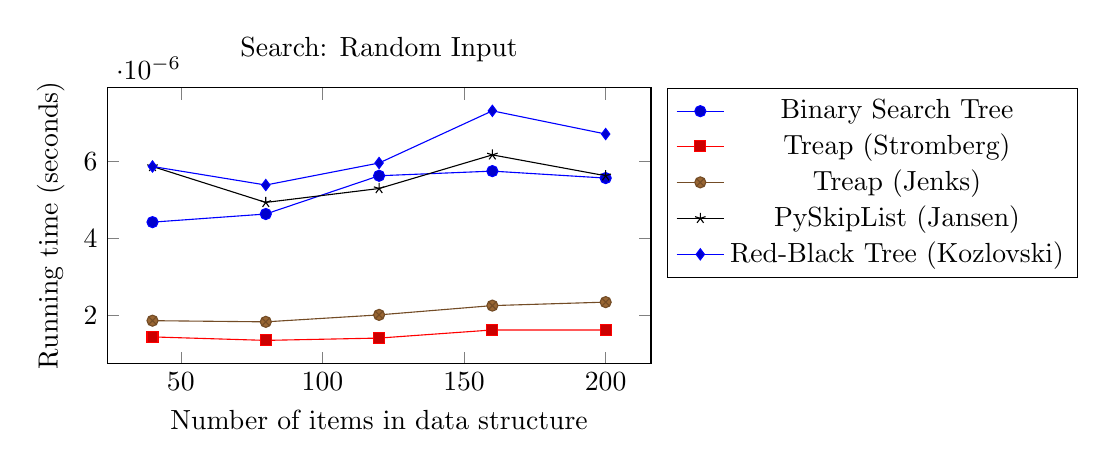
\begin{tikzpicture}
        \begin{axis}[
            xlabel={Number of items in data structure},
            ylabel={Running time (seconds)},
            title={Search: Random Input},
            width=0.7\textwidth,
            height=2in,
            legend pos=outer north east
        ]
		\addplot coordinates {
			(40, 4.427277450250178e-06)
			(80, 4.638100185977434e-06)
			(120, 5.63197879725752e-06)
			(160, 5.752448931956033e-06)
			(200, 5.571743729906875e-06)
		};
		\addplot coordinates {
			(40, 1.445641616407145e-06)
			(80, 1.3552890153839537e-06)
			(120, 1.4155240827345984e-06)
			(160, 1.626346818459079e-06)
			(200, 1.626346818459079e-06)
		};
		\addplot coordinates {
			(40, 1.867287087858882e-06)
			(80, 1.8371695541835597e-06)
			(120, 2.017874756235494e-06)
			(160, 2.2588150256380725e-06)
			(200, 2.3491676266612638e-06)
		};
		\addplot coordinates {
			(40, 5.872919066660098e-06)
			(80, 4.939275522727882e-06)
			(120, 5.300685926828974e-06)
			(160, 6.174094403410546e-06)
			(200, 5.631978797254744e-06)
		};
		\addplot coordinates {
			(40, 5.872919066657323e-06)
			(80, 5.391038527854941e-06)
			(120, 5.96327166768329e-06)
			(160, 7.318560683067244e-06)
			(200, 6.716210009560797e-06)
		};
        \legend{Binary Search Tree, Treap (Stromberg), Treap (Jenks), PySkipList (Jansen), Red-Black Tree (Kozlovski)}
        \end{axis}
    \end{tikzpicture}
    \caption{Average of 10 operations, benchmarked every 40, starting at 40.}
\end{figure}